\section{Výstup sítí}
\label{sec:Chapter46}
\subsection{Výstupní vrstva}
Jak bylo již řečeno v předchozích sekcích o návrhů sítí U-Net, U-Net++ a U-Net STN, finální vrstvou je vždy konvoluční operace $1\times1$ s aktivační funkcí sigmoid, generující mapu příznaků ekvivalentní velikosti jako je vstupní obraz. V této práci používáme 11 tříd pro lokalizaci, kde lokalizace probíhá na každém jednotlivém filtru pro daný kanál separátně, čili velikost výstupu je velikost vstupního obrázku (díky odsazení typu same padding) o hloubce 11 kanálů.

Aktivační funkce sigmoid je funkce, která se používá v neuronových sítích k převodu vstupních hodnot na hodnoty v rozmezí 0 a 1. Je definována vzorcem:

\begin{equation}
\sigma(x) = \frac{1}{1+e^{-x}},
\end{equation}

kde $e$ je základ přirozeného logaritmu a $x$ je vstupní hodnota. Tato funkce je obzvláště užitečná v úloze pro lokalizaci. Každý kanál tedy můžeme chápat jako binární softmax klasifikátor na úrovni pixelů, kde \enquote{pravděpodobnost} výskytu daného klíčového bodu je hodnota daného pixelu.

\begin{figure}[H]
    \centering
    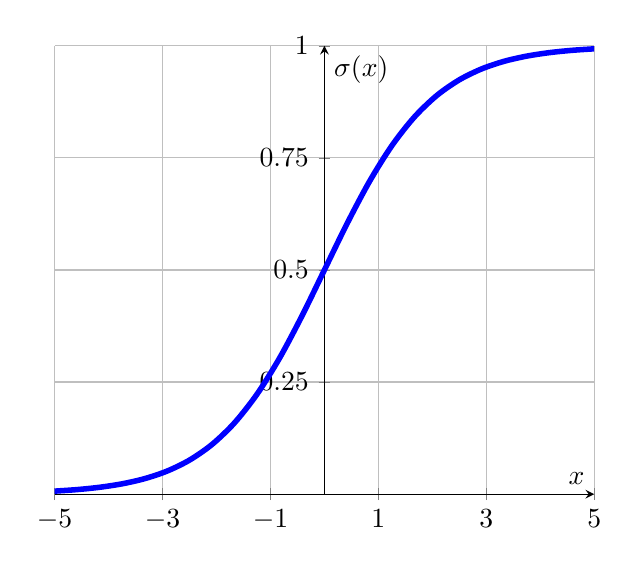
\begin{tikzpicture}
    \begin{axis}[
        axis lines=middle,
        xlabel={$x$},
        ylabel={$\sigma(x)$},
        ymin=0, ymax=1,
        xmin=-5, xmax=5,
        xtick={-5,-3,...,5},
        ytick={0,0.25,...,1},
        grid=major,
    ]
    \addplot[blue,smooth, line width=2pt] {1/(1+exp(-x))};
    \end{axis}
    \end{tikzpicture}
    \caption[Aktivační funkce sigmoid]{Aktivační funkce sigmoid}
    \label{fig:sigmoid}
\end{figure}

Toto vede k možnosti jednoduše provést lokální klasifikaci na jednotlivých kanálech, a to s pomocí maximální nalezené hodnoty na výstupním kanálu (což je typicky z praktického hlediska i hledaná pozice klíčového bodu). Například výstupní kanál s maximální hodnotou 0.8 vykazuje silnou pravděpodobnost výskytu klíčového bodu na daném kanálu, na rozdíl od kanálu s max. hodnotou 0.3.

\subsection{Reprezentace klíčových bodů}

Jako reprezentaci klíčových bodů na výstupu sítě si v tomto nastavení volíme reprezentaci Gaussovy funkce ve 2D prostoru. Gaussova funkce působí jako přirozený kandidát pro aktivační funkci sigmoid. Tato reprezentace má svou maximální hodnotu o hodnotě 1 ve svém středu, kde se nachází náš klíčový bod v době tréninku. Gaussovou funkci pro výpočet hodnot na 2D skalární mapě jako tzv. ground truth pro trénink výstupních kanálů můžeme zapsat takto:

\begin{equation}
    G(x, y) = a \exp\left(-\frac{(x - c_x)^2 + (y - c_y)^2}{2\sigma^2}\right)
\end{equation}
kde $a$ je amplitudový faktor Gaussovy funkce, $x$ a $y$ jsou pozice na 2D skalárním poli, $(c_x, c_y)$ označují souřadnice středu klíčového bodu a $\sigma$ udává směrodatnou odchylku, která ovlivňuje rozptyl Gaussovy funkce. Parametry Gaussovy funkce si volíme jako následující hodnoty pro adekvátní rozptyl na výstupních kanálech: 
\begin{itemize}
    \item pro $128 \times 128$ snímky -- $a=1$, $\sigma=$ 5.0
    \item pro $256 \times 256$ snímky -- $a=1$, $\sigma=$ 10.0
\end{itemize}

\begin{figure}[H]
\centering
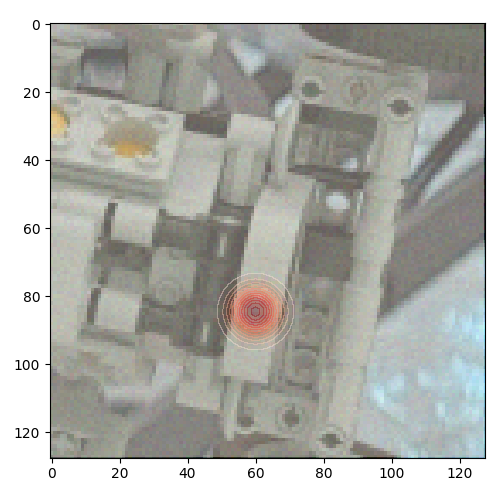
\includegraphics[width=0.3\textwidth,keepaspectratio]{Figures/kp_examples/kp_example_00.png}
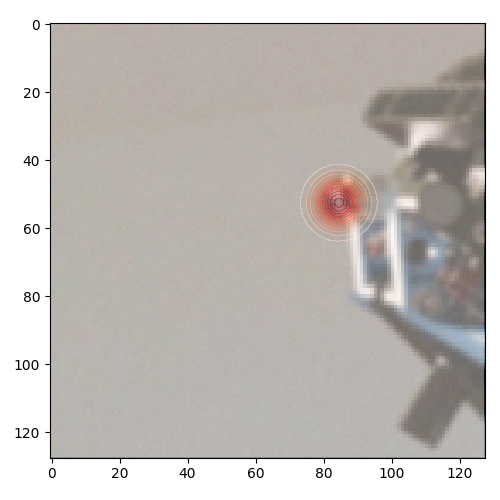
\includegraphics[width=0.3\textwidth,keepaspectratio]{Figures/kp_examples/kp_example_01.png}
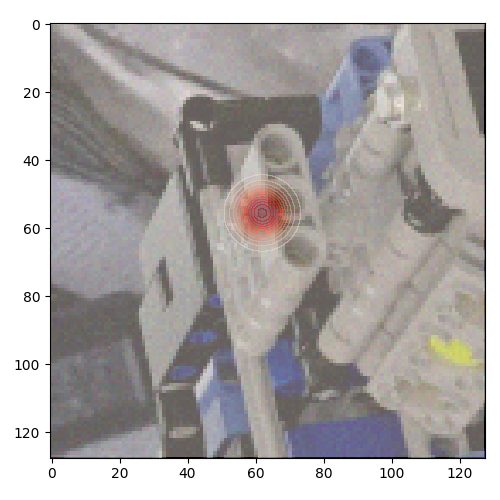
\includegraphics[width=0.3\textwidth,keepaspectratio]{Figures/kp_examples/kp_example_02.png}
\caption[Příklad aplikace Gaussovy funkce na snímky s klíčovým bodem]{Příklad aplikace Gaussovy funkce na augmentované snímky s klíčovým bodem.}
\label{fig:kp_examples}
\end{figure}

Během experimentálních trénincích nevyskytujících se ve finálních evaluacích jsme pracovali i s premisí odebrání ReLU aktivační funkce na posledním bloku dekodéru těsně před aplikací sigmoid aktivační funkce. Tato premise se neobhájila a vyšlo najevo, že představení linearity v předposlední konvoluční operaci má detrimentální účinky na lokalizační přesnost sítě. MOŽNÁ DÁT DO DALŠÍ KAPITOLY.
\endinput